%% LyX 2.3.0 created this file.  For more info, see http://www.lyx.org/.
%% Do not edit unless you really know what you are doing.
\documentclass[english]{cinc-abstract}
\usepackage[T1]{fontenc}
\usepackage[latin9]{inputenc}
\usepackage{graphicx}

\makeatletter
%%%%%%%%%%%%%%%%%%%%%%%%%%%%%% User specified LaTeX commands.
% -*- Mode:TeX -*-

\makeatother

\usepackage{babel}
\begin{document}

\title{Action Potential Modelling in Isolated Rat Hearts during Hypokalemia}

\author{Mariano Llamedo, Emiliano Diez\\
\mbox{}\\
GIBIO, National Technological University, Buenos Aires, Argentina\\
Institute of Physiology, Medical School, National University of Cuyo,
Mendoza, Argentina\\
}

\maketitle
\emph{Introduction}: Hypokalemia is the most common electrolyte abnormality
encountered in clinical practice and enhances the propensity for ventricular
fibrillation. An automatic methodology for modeling rats action potential
was developed in this work.

\emph{Materials and Methods}: Isolated rat hearts underwent low K+
perfusion (1 mEq/L) in 4 groups: 1) Mel, $100\,\mathrm{\mu M}$ melatonin;
2) Luz, luzindole $5\,\mathrm{\mu M}$ a melatonin receptor blocker;
3) Mel+Luz melatonin+luzindole; or 4) Control. The ECG and epicardial
action potential (AP) were recorded and automatically analyzed with
an \emph{ad-hoc} algorithm also presented in this conference. The
AP was modeled by morphological and temporal features. The activation
delay between the start of the QRS complex and the AP was also calculated.

\emph{Results}: The heart rhythm, PR and QT interval are presented
for the analyzed groups. Further measurements and statistical differences
are being analyzed.

\emph{Discussion}: Hypokalemia contributes to reducing survival of
cardiac patients and increases the incidence of arrhythmic death.
Melatonin protects against several cardiovascular diseases and exhibits
antiarrhythmic potential. This effect was related to up-regulation
of myocardial connexin-43, the main protein responsible for electrical
coupling. The automatic methodology presented in this work may allow
further research in these mechanisms by increasing the size of the
experimentation groups, or the signals involved in the experimentation.


\begin{wrapfigure}{r}{1\textwidth}
  \vspace{-3mm}
  \begin{center}

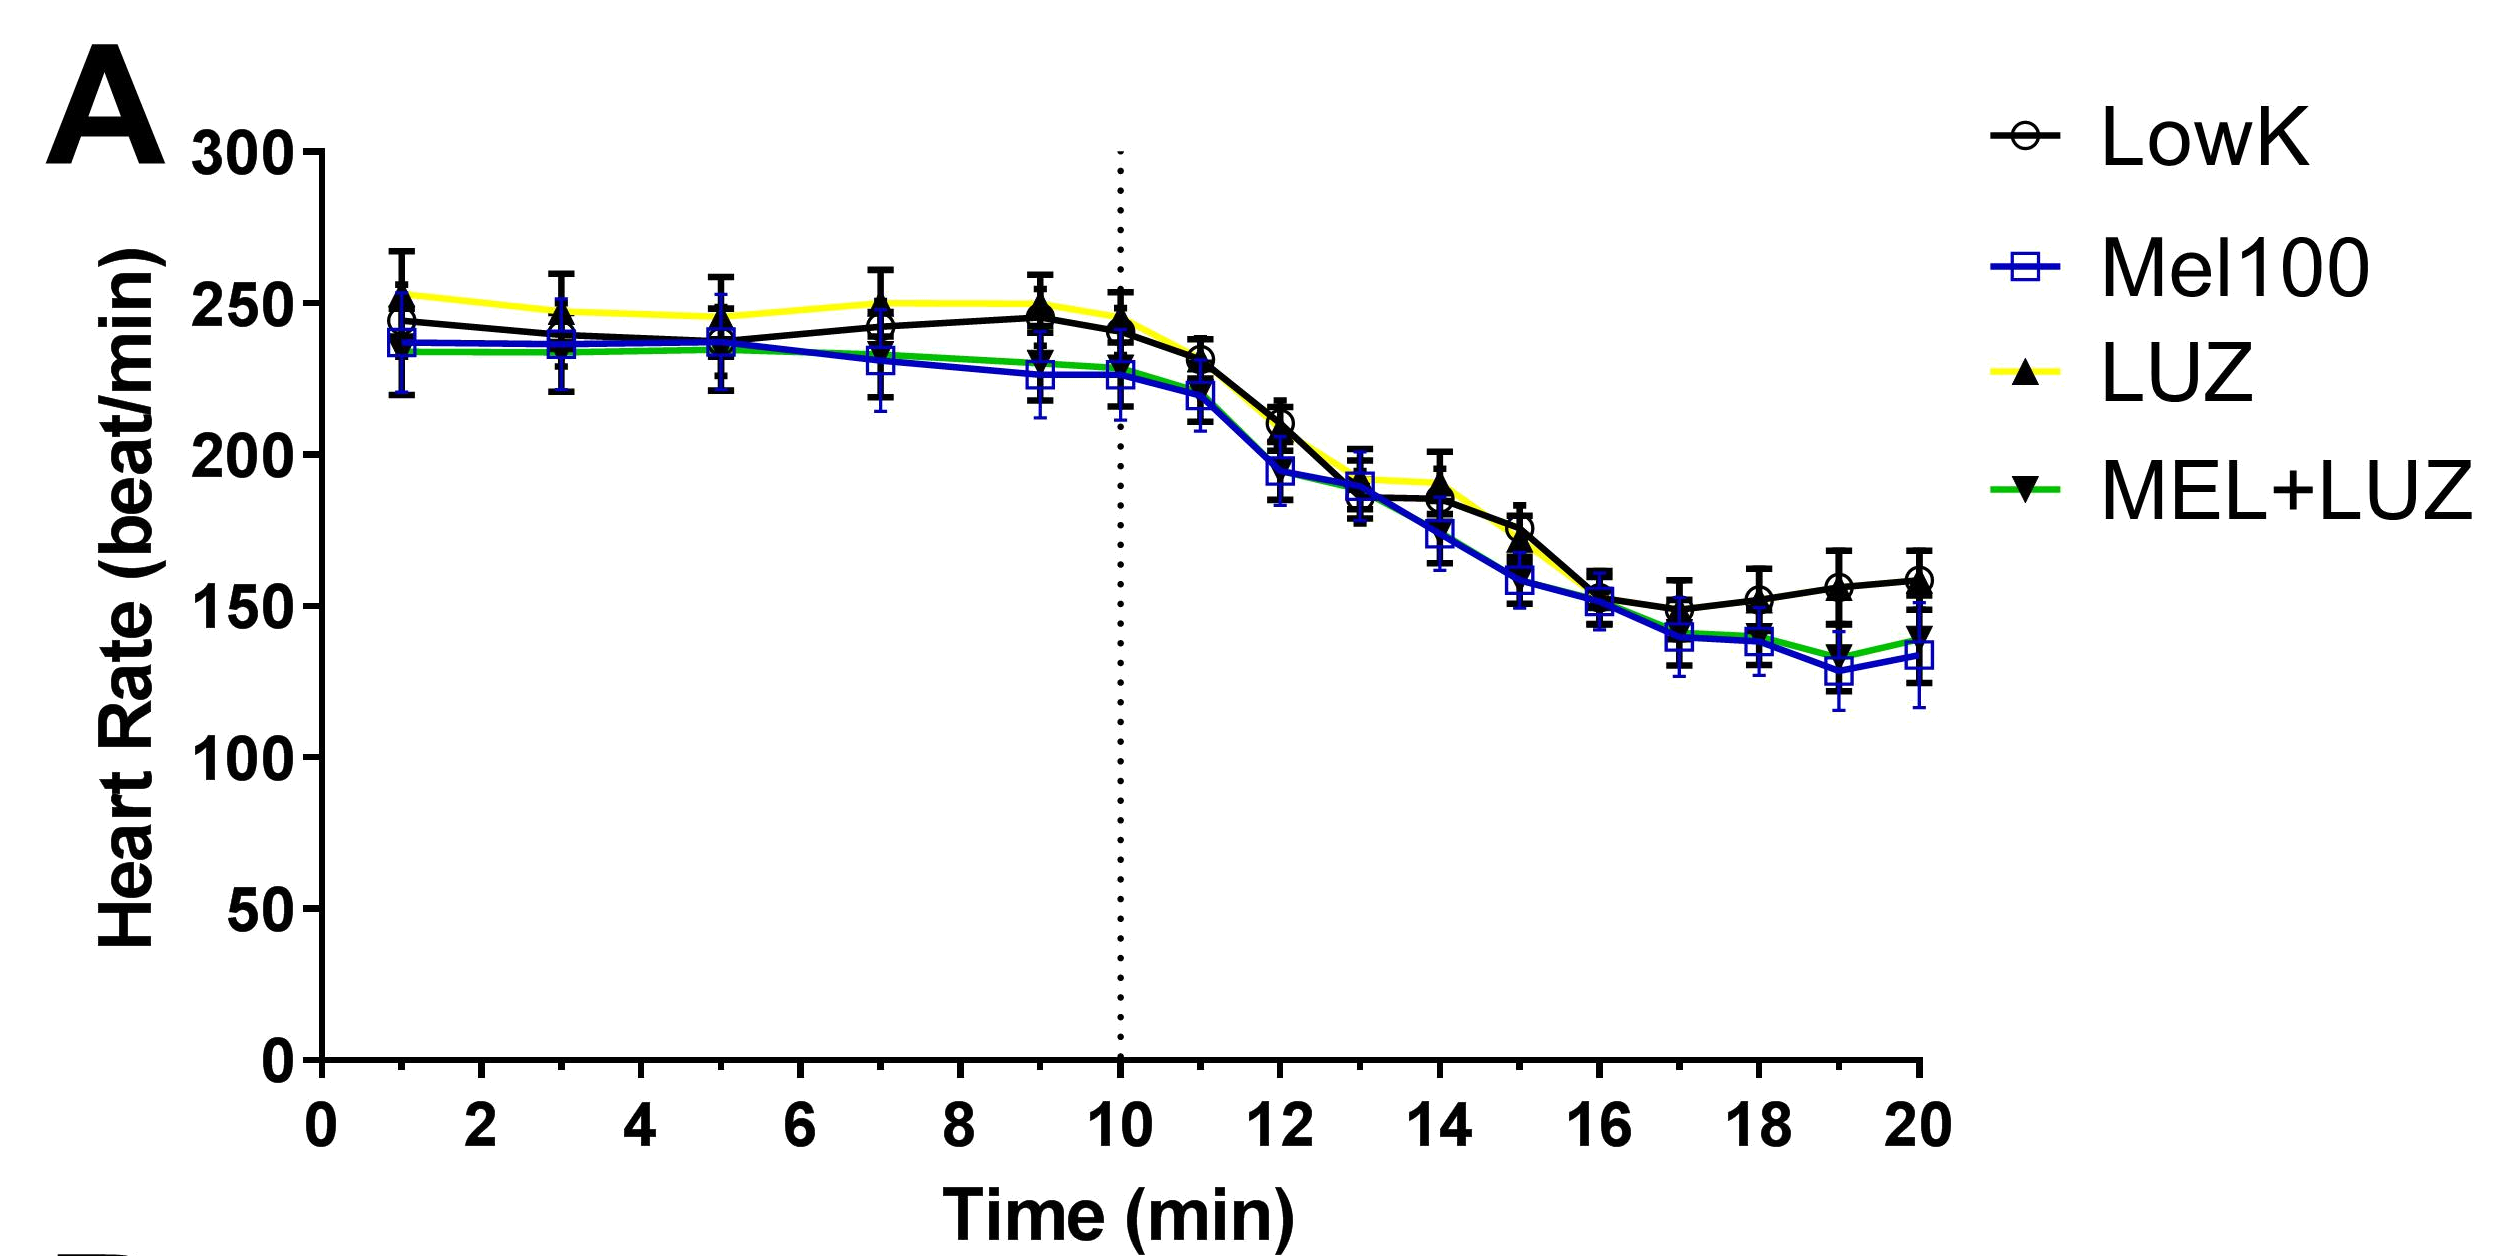
\includegraphics[width=0.33\textwidth]{hr}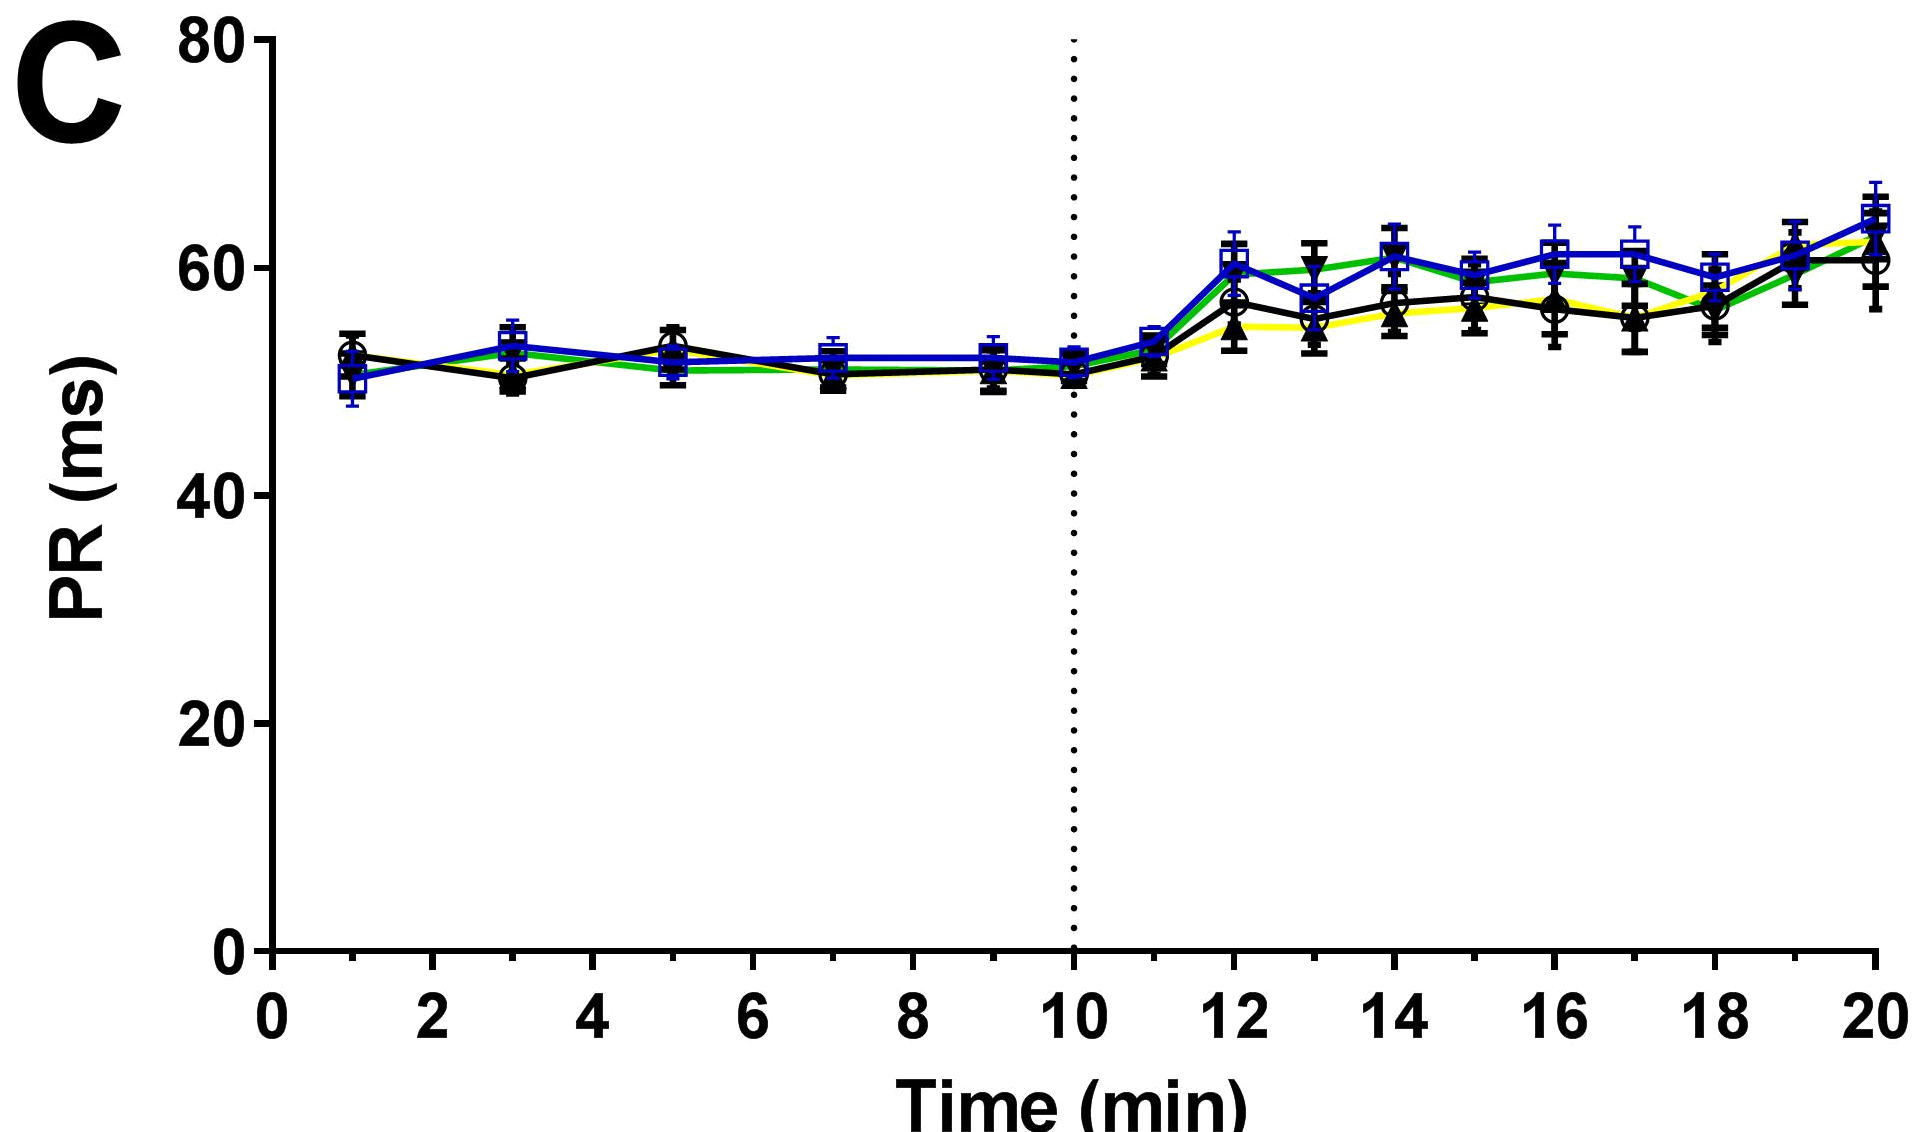
\includegraphics[width=0.33\textwidth]{PR}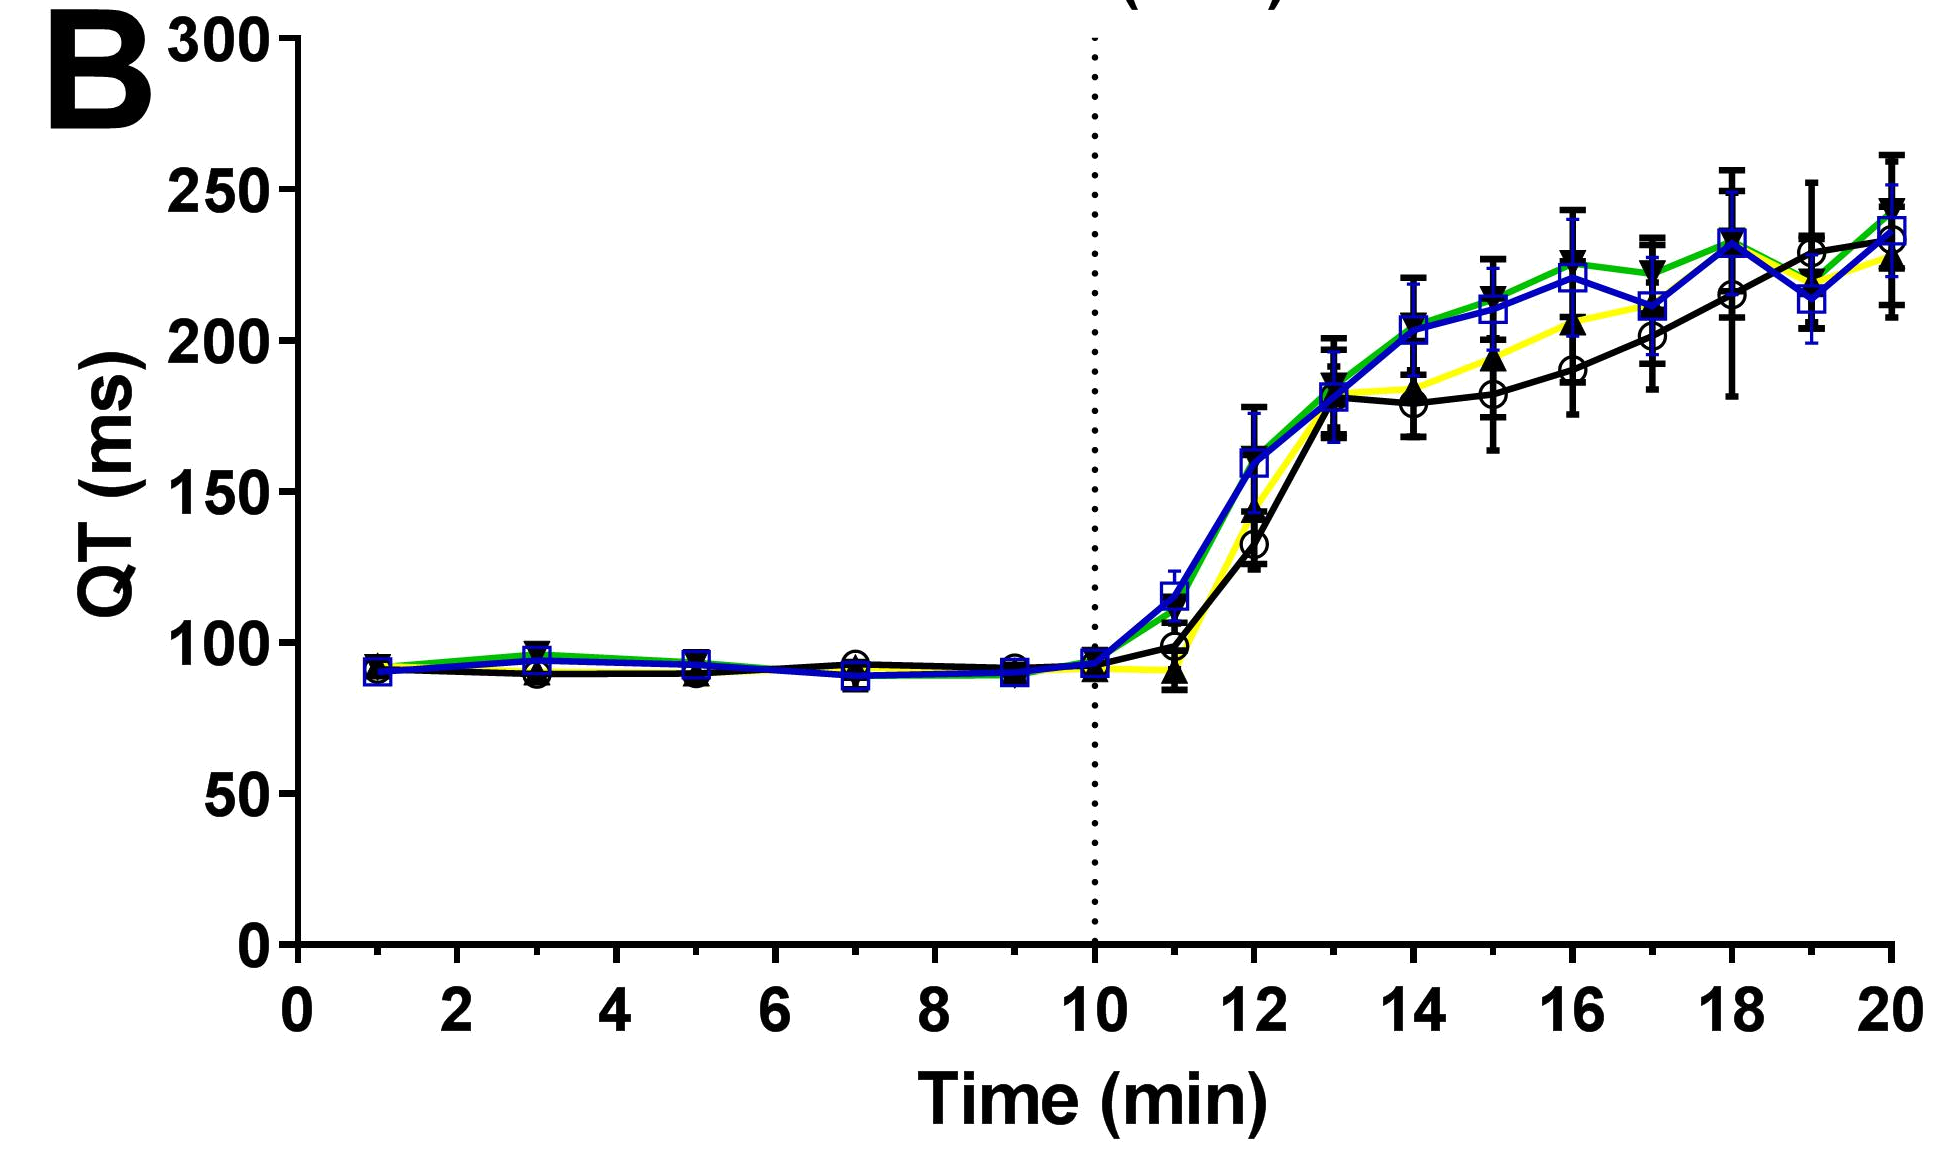
\includegraphics[width=0.33\textwidth]{qt}

 \raggedright     
 Heart rhythm, PR and QT intervals for the studied groups.
 \end{center}
 \vspace{-3mm}
\end{wrapfigure}
\end{document}
